\section{Results}
\label{sec:results}

We have tested our system on a large number of scenes, including the 32 scenes available
at Bitterli's rendering resources website~\cite{resources16}. 
%We validated our system's conversion using scenes from Bitterli's 32 resources 
%\cite{resources16}. 
Here, we include a few examples that explore different 
types of materials and bump maps, 3D meshes and primitive shapes, image and 
primitive textures, and area light sources and environment lighting. They include most elements typically found in scenes used by physically-based rendering systems.  The time required to convert a scene is about 0.5 seconds on a typical PC (Intel i5 3.8 GHz).
% 
%We chose scenes that provided a wide variety of directives 
%in order to cover most commonly used directives. These scenes include: different 
%types of materials and bump maps; 3D meshes and primitive shapes; image and 
%primitive textures; area and environment lighting. 
%
The scenes were rendered using Mitsuba 0.5.0, PBRT v3, and LuxRender v1.6 on 
Ubuntu 14.04 LTS. All scenes were rendered using between 5,000 and 8,000 samples per pixel (spp). For any given scene,
the same number of samples per pixel was used with all rendering systems. 

Figure~\ref{fig:teaser} shows a coffee maker containing different kinds of materials, including glass, plastic, and metal, as well as textures. The input scene description was provided in the format for PBRT v3, whose rendering is shown on the left. The images at the center and on the right were produced by Mitusuba and LuxRender, respectively, from scene representations automatically converted by our system from the input scene file. Note how the object details have been faithfully preserved in these renderings.

The \textit{The Wooden Staircase} scene (Figure~\ref{fig:staircase} explores the use of textures and geometric details. This scene was originally modeled for 

We obtained interesting results with \textit{The Wooden Staircase} (Figure 
\ref{fig:staircase}, \textit{Utah Teapot} (Figure \ref{fig:teapot}), 
\textit{Coffee Maker} (Figure \ref{fig:teaser}) and Glass of Water (Figure 
\ref{fig:glass-of-water}). We reached a high degree of visual similarity between 
the original and the converted scenes, which was our goal.

We can observe some difference in coloring between the image rendered by Mitsuba 
(center) and the ones rendered by other two renderers in Figure 
\ref{fig:dining-room}. This particular scene uses a distant environment light to 
emulate the sun. In Mitsuba, this directive is implemented using the technique 
described in \cite{Preetham}, which produces a warm-colored, distant light source. In 
PBRT and LuxRender, this directive is implemented simply as a distant white 
light, which produces the difference shown in the results.

\begin{figure}
\centering

\subfloat[LuxRender]{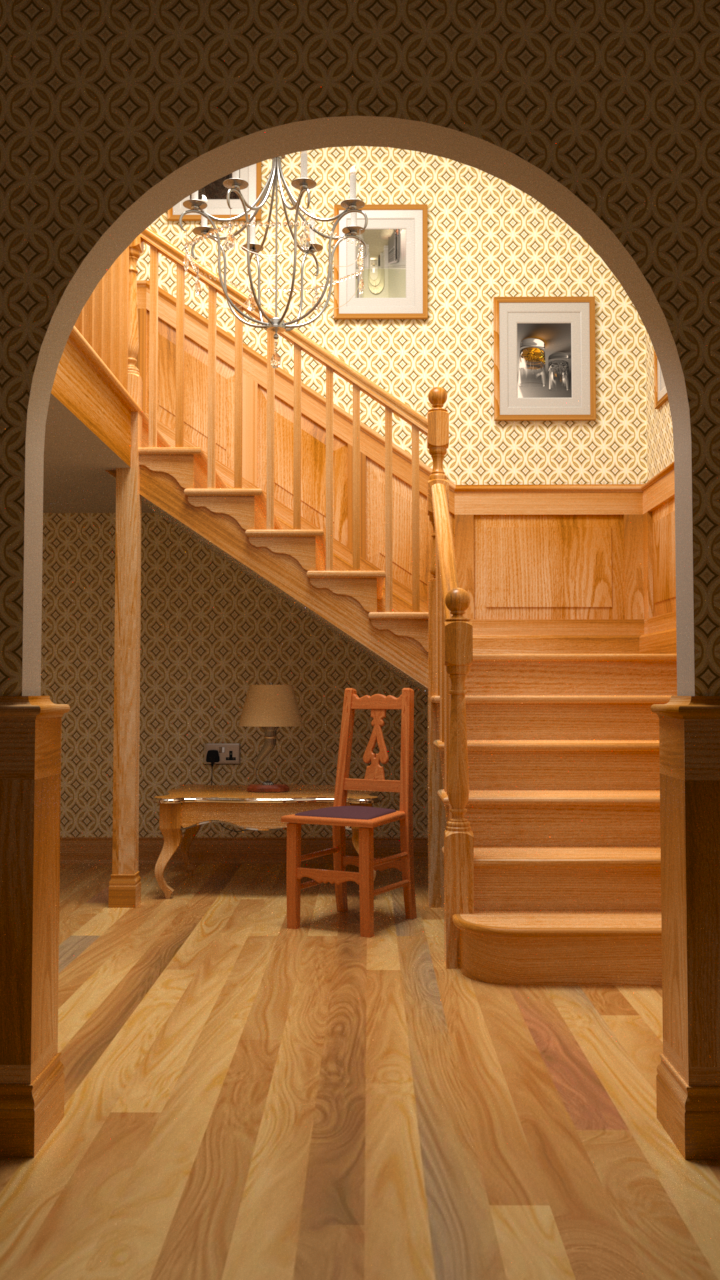
\includegraphics[width=0.32\linewidth]{figs/4_results/staircase/1_from_lux.png}
	\label{staircase_Lux}
}
\subfloat[PBRT v3]{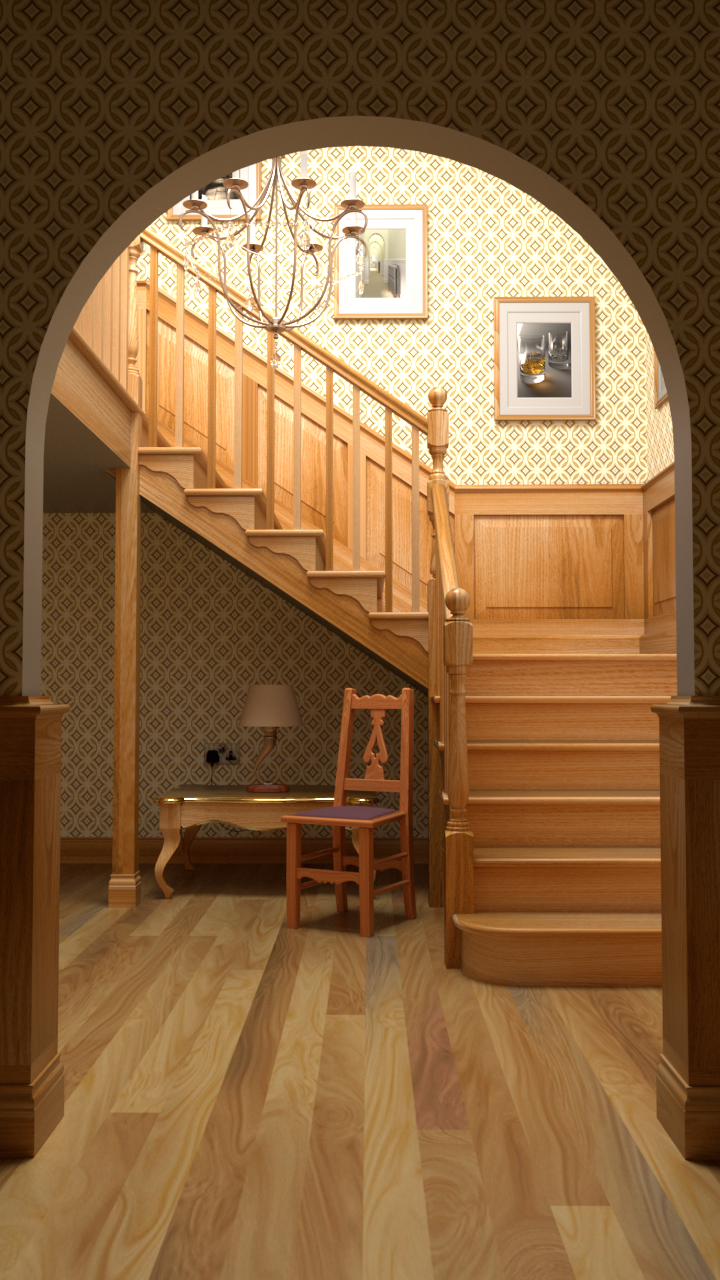
\includegraphics[width=0.32\linewidth]{figs/4_results/staircase/3_to_pbrt.png}
	\label{staircase_PBRT}
}
\subfloat[Mitsuba]{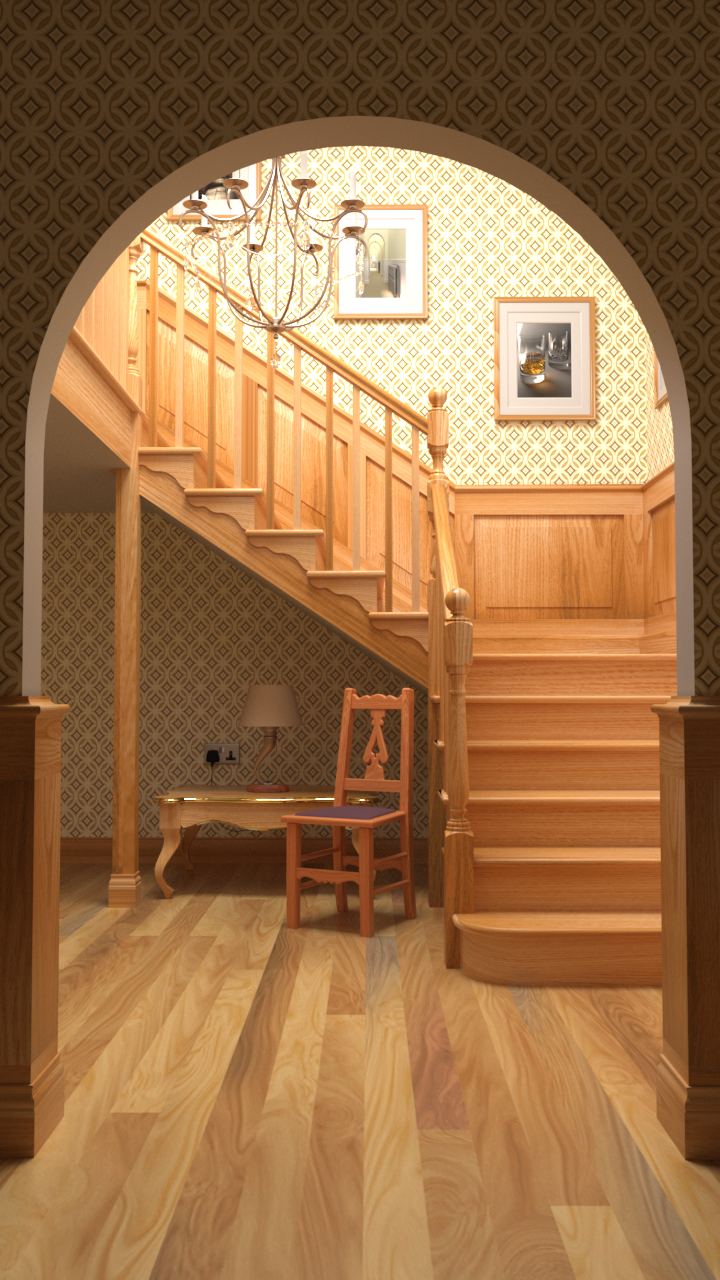
\includegraphics[width=0.32\linewidth]{figs/4_results/staircase/2_to_mitsuba.png}
	\label{staircase_Mitsuba}
}
\caption{\textit{The Wooden Staircase} scene. Input scene description for LuxRender (a).
Renderings produced by PBRT v3 (b) and Mitsuba (c),
from scene descriptions converted by our system. }
\label{fig:staircase}
\end{figure}

\begin{figure*}
\centering

\subfloat[LuxRender]{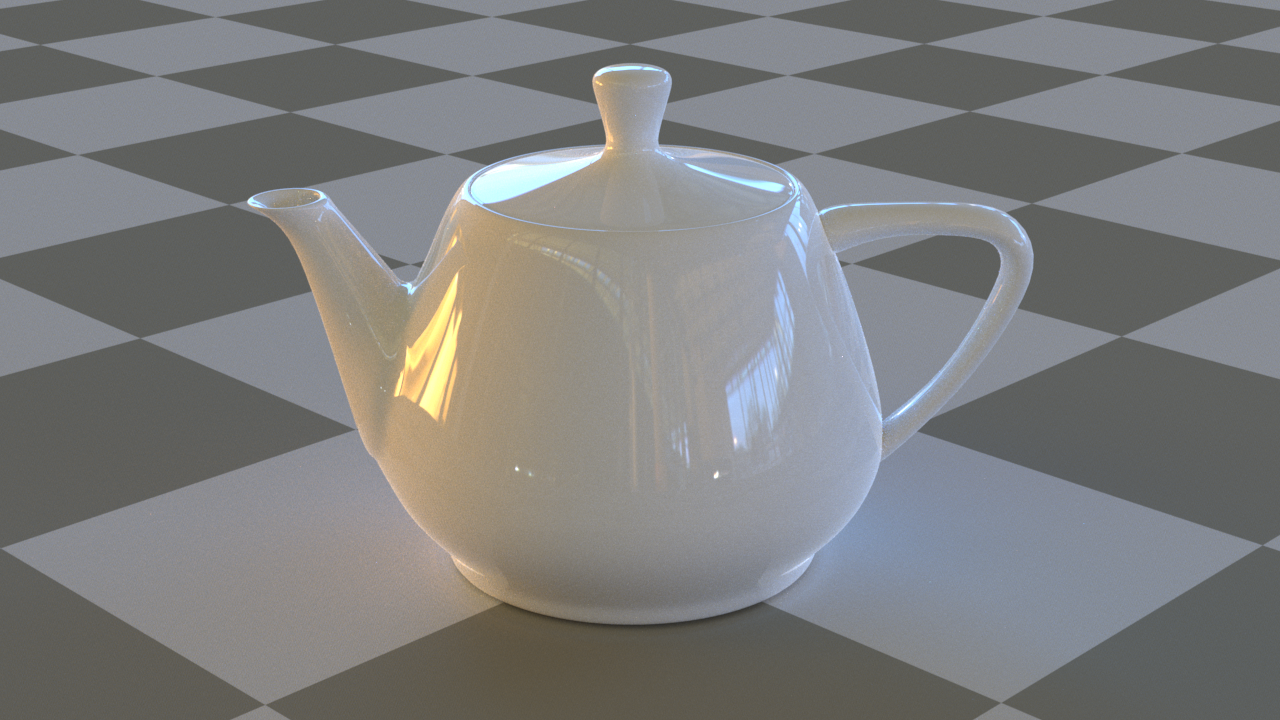
\includegraphics[width=0.32\linewidth]{figs/4_results/teapot/1_from_lux.png}
	\label{teapot_Lux}
}
\subfloat[PBRT v3]{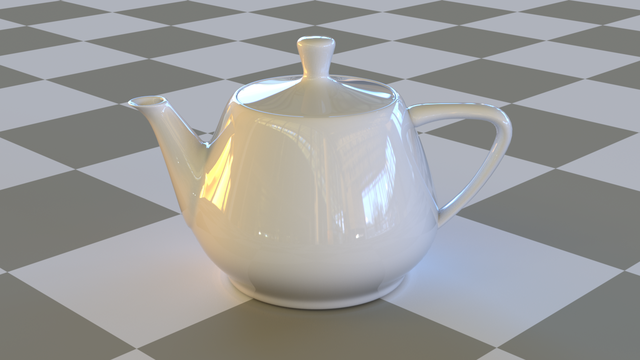
\includegraphics[width=0.32\linewidth]{figs/4_results/teapot/3_to_pbrt.png}
	\label{teatpot_PBRT}
}
\subfloat[Mitsuba]{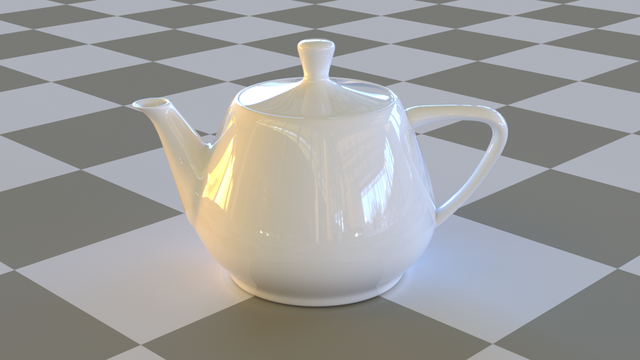
\includegraphics[width=0.32\linewidth]{figs/4_results/teapot/2_to_mitsuba.png}
	\label{teapot_Mitsuba}
}
%
%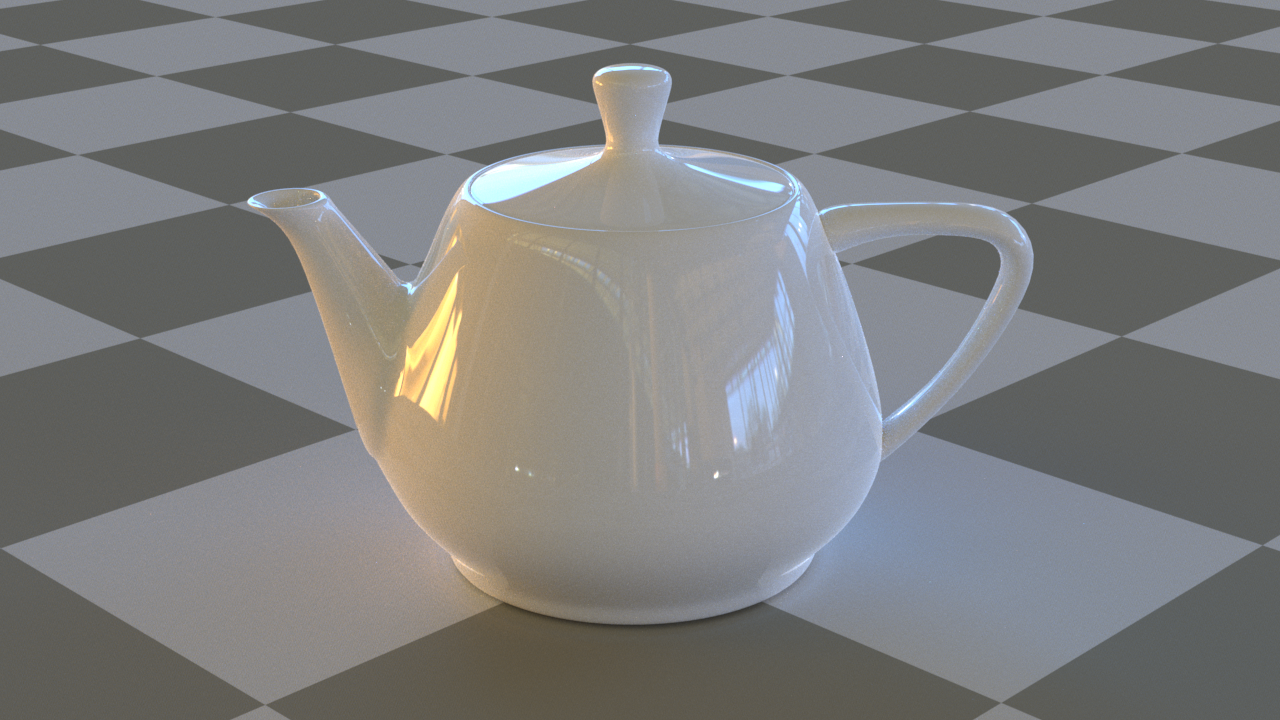
\includegraphics[width=0.32\linewidth]{figs/4_results/teapot/1_from_lux.png}
%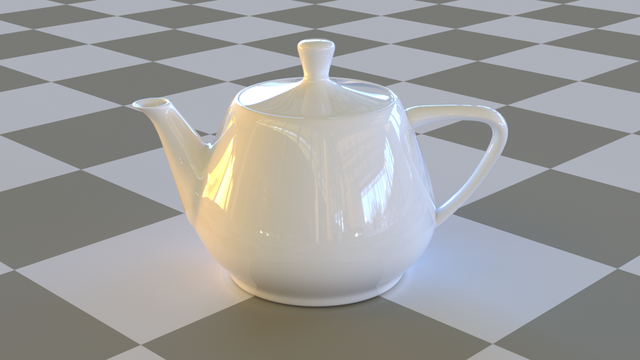
\includegraphics[width=0.32\linewidth]{figs/4_results/teapot/2_to_mitsuba.png}
%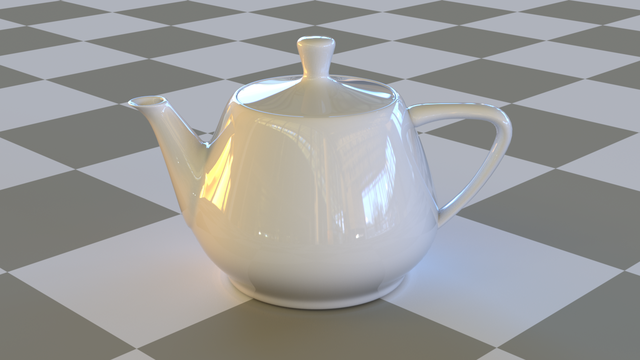
\includegraphics[width=0.32\linewidth]{figs/4_results/teapot/3_to_pbrt.png}
\caption{\textit{Teapot} scene. Input scene description for LuxRender (a).	Renderings produced by PBRT v3 (b) and Mitsuba (c),
	from scene descriptions converted by our system.}
\label{fig:teapot}
\end{figure*}

\begin{figure}
\centering
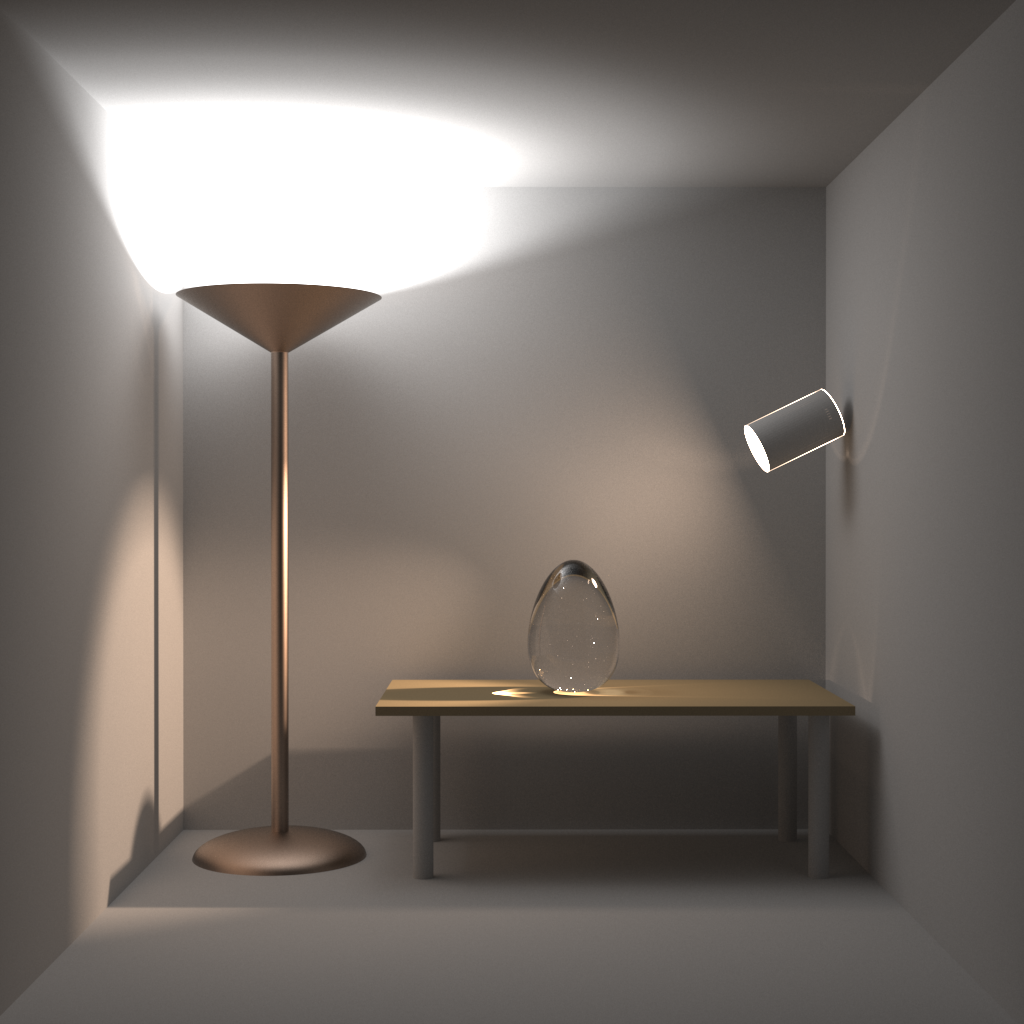
\includegraphics[width=0.325\linewidth]{figs/4_results/veach-bidir/1_from_mitsuba.png}
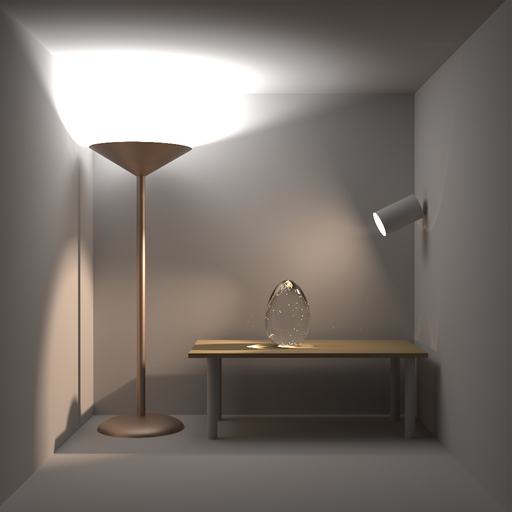
\includegraphics[width=0.325\linewidth]{figs/4_results/veach-bidir/2_to_pbrt.png}
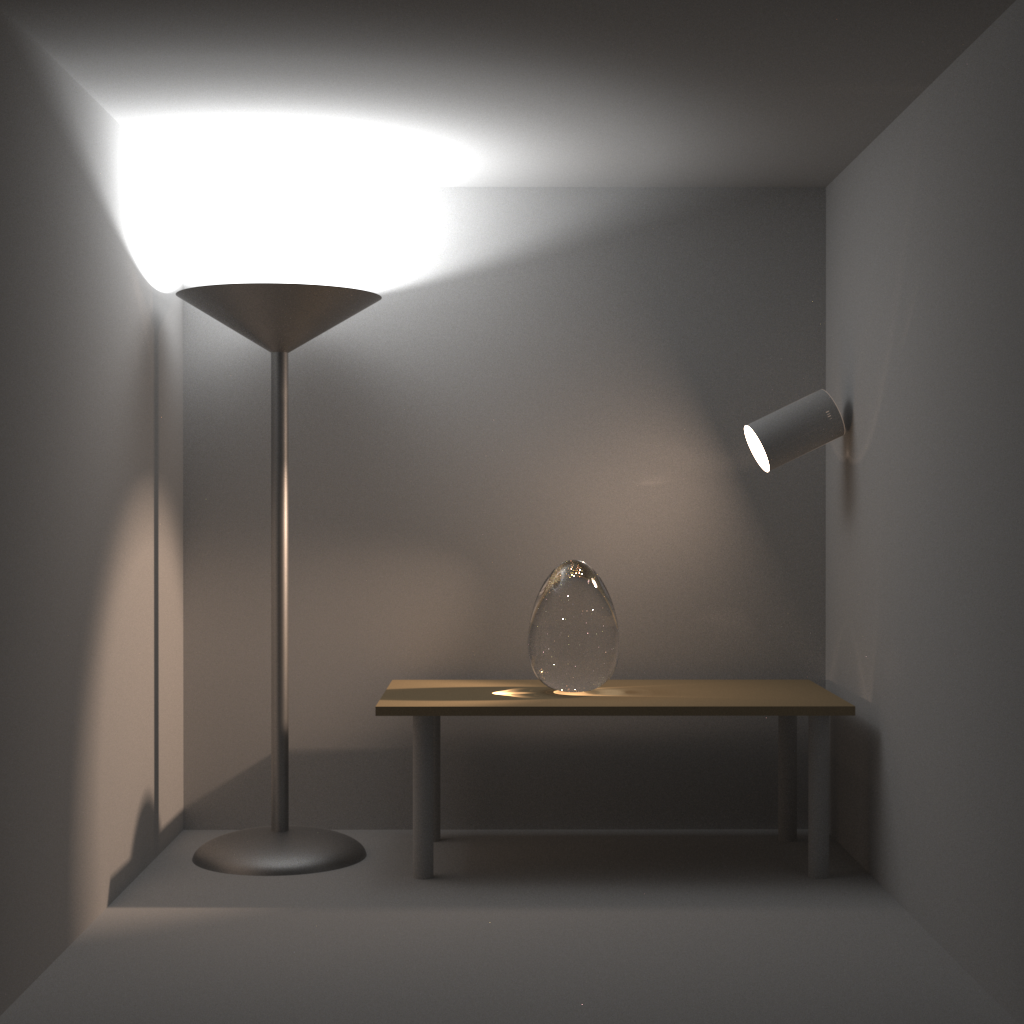
\includegraphics[width=0.325\linewidth]{figs/4_results/veach-bidir/3_to_lux.png}
%\vspace{-0.2cm}
\subfloat[Mitsuba]{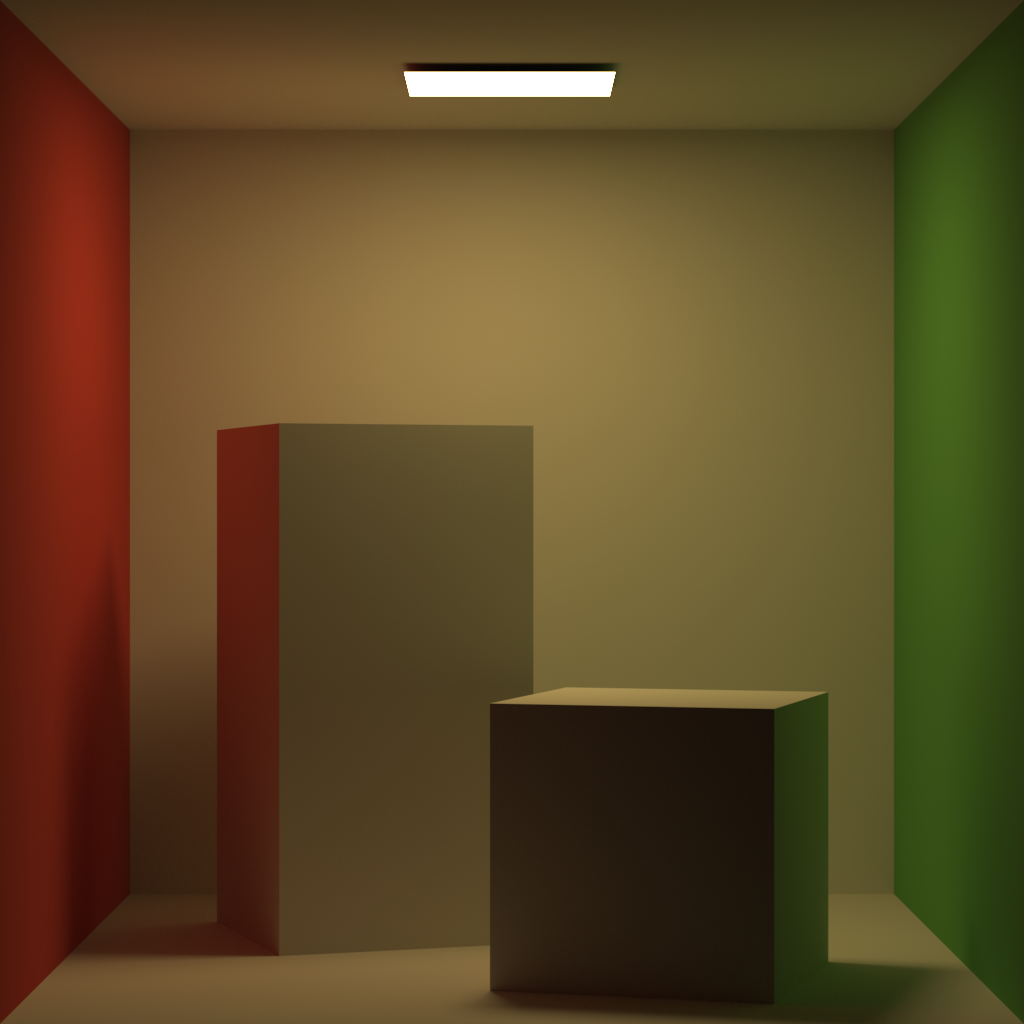
\includegraphics[width=0.325\linewidth]{figs/4_results/cornell-box/1_from_mitsuba.png}
}	
\subfloat[PBRT v3]{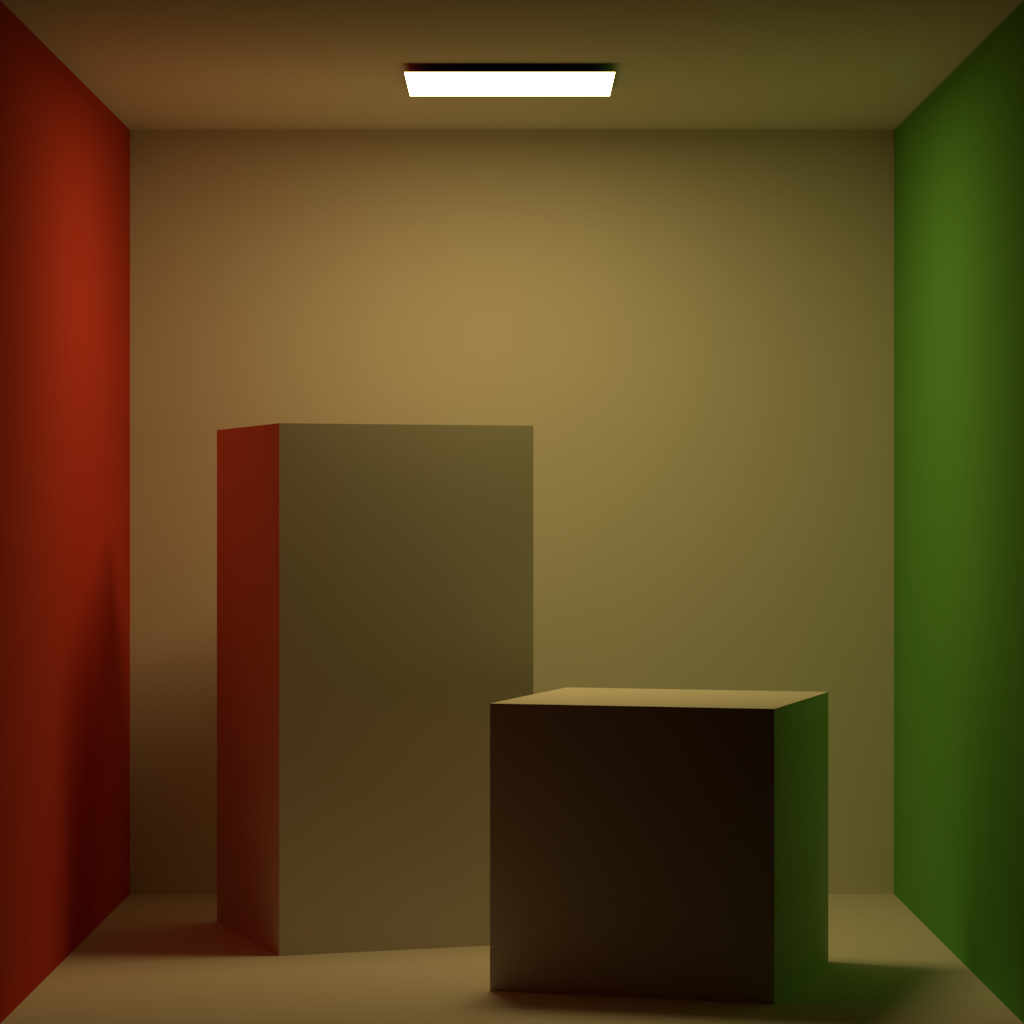
\includegraphics[width=0.325\linewidth]{figs/4_results/cornell-box/2_to_pbrt.png}
}	
\subfloat[LuxRender]{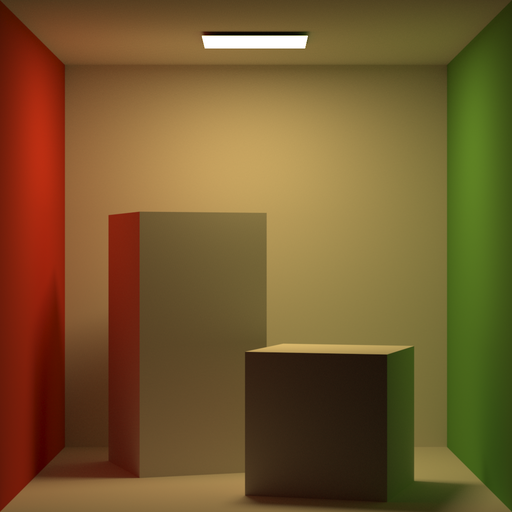
\includegraphics[width=0.325\linewidth]{figs/4_results/cornell-box/3_to_lux.png}}
\caption{\textit{Veach, Bidir Room} (top) and \textit{Cornell Box} (bottom). Input scene descriptions for 
 Mitsuba (a). Renderings produced by PBRT v3 (b) and LuxRender (c),
 from scene descriptions converted by our system.}
\label{fig:veach-bidir}
\end{figure}

\begin{figure}
\centering
\subfloat[LuxRender]{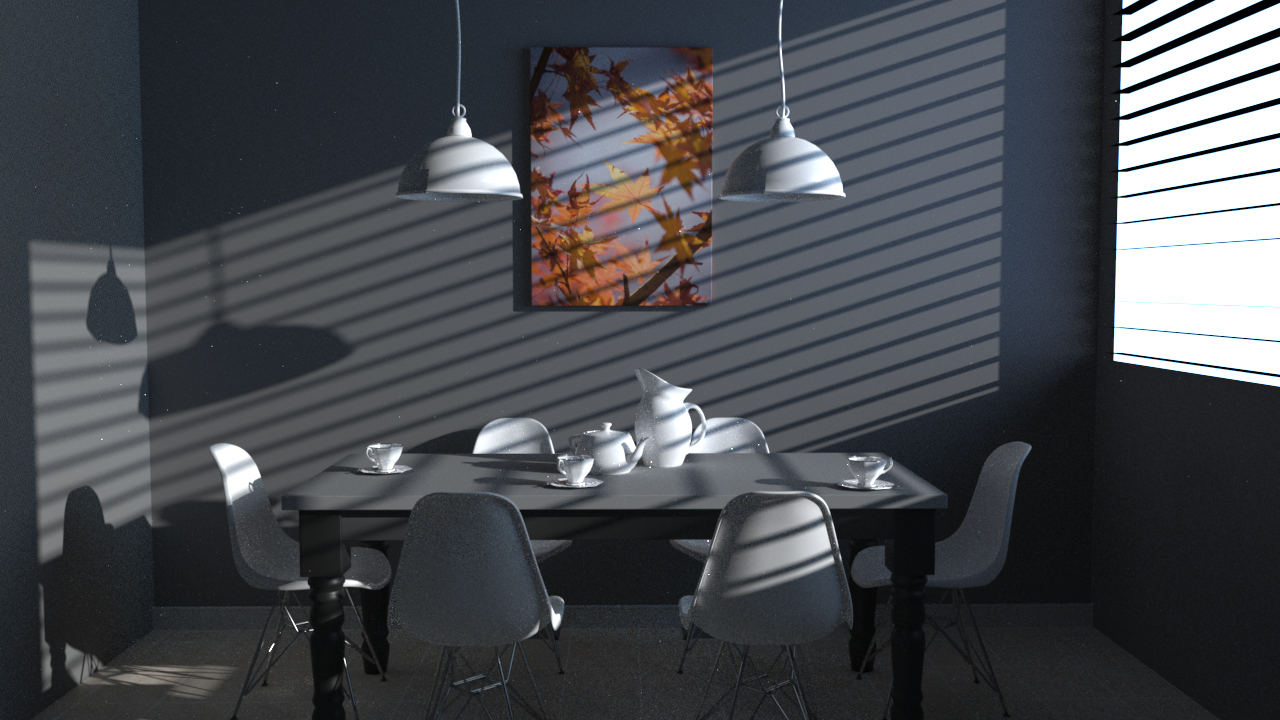
\includegraphics[width=0.32\linewidth]{figs/4_results/dining_room/1_from_lux.png}
	\label{breakfast_Lux}	
}	
\subfloat[PBRT v3]{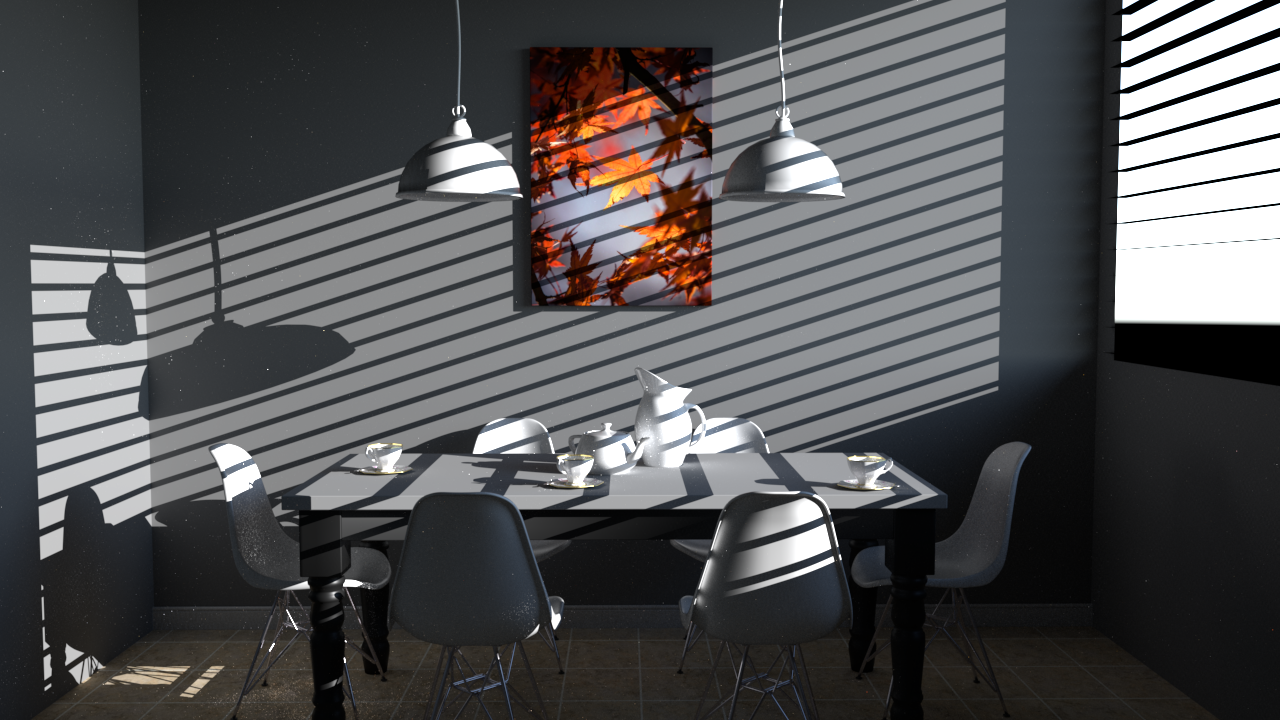
\includegraphics[width=0.32\linewidth]{figs/4_results/dining_room/3_to_pbrt.png}
	\label{breakfast_PBRT}		
}	
\subfloat[Mitsuba]{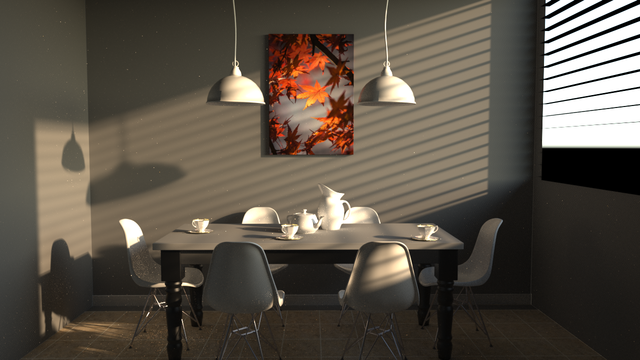
\includegraphics[width=0.32\linewidth]{figs/4_results/dining_room/2_to_mitsuba.png}
		\label{breakfast_Mitsuba}	
}	
\caption{\textit{The Breakfast Room} scene. Input scene description for LuxRender (a).
	Renderings produced by PBRT v3 (b) and Mitsuba (c),
	from scene descriptions converted by our system. }
\label{fig:dining-room}
\end{figure}

\begin{figure}
\centering
\subfloat[PBRT v3]{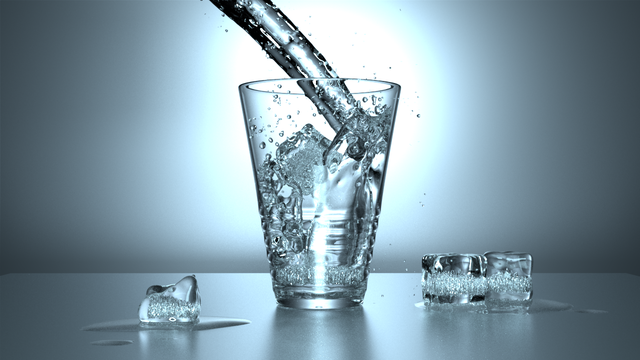
\includegraphics[width=0.32\linewidth]{figs/4_results/glass_of_water/1_from_pbrt.png}
	\label{glass_PBRT}		
}	
\subfloat[LuxRender]{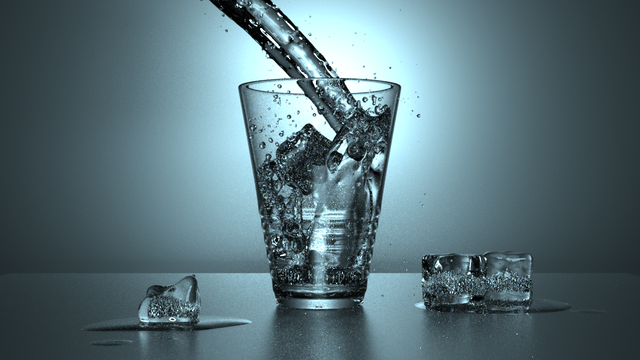
\includegraphics[width=0.32\linewidth]{figs/4_results/glass_of_water/2_to_lux.png}
	\label{glass_Lux}		
}	
\subfloat[Mitsuba]{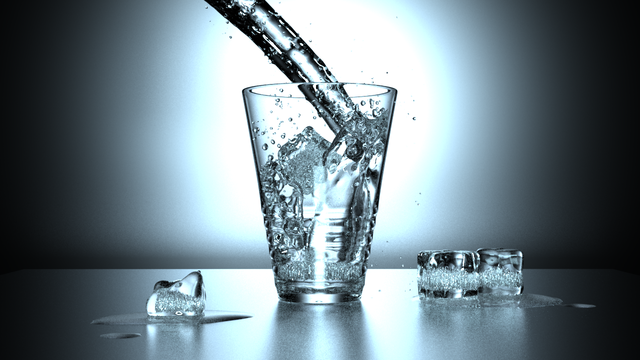
\includegraphics[width=0.32\linewidth]{figs/4_results/glass_of_water/3_to_mitsuba.png}
	\label{glass_Mitsuba}		
}	
\caption{\textit{Glass of Water}. Input scene description for PBRT v3 (a).
	Renderings produced by LuxRender (b) and Mitsuba (c),
	from scene descriptions converted by our system. } 
\label{fig:glass-of-water}
\end{figure}

\subsection{Limitations}
In order to minimize scope issues, we restricted the number of directives 
interpreted by our system. Generally speaking, directives present in only one 
renderer that had no correspondent in the other two renderers were not 
incorporated. That was the case, for instance, for Mitsuba-only materials like 
\textit{phong} or \textit{blendbsdf}. 

We chose not to interpret and convert hair or participating media (volumes, such 
as water or fog) for this PoC. We also did not convert the color for metal 
materials in LuxRender given the issues discussed in \ref{systemarch}. The 
latter can be observed in Figure \ref{fig:veach-bidir} - we can see the lack of a 
copper color on the lamp in the image rendered by LuxRender.




